%%%%%%%%%%%%%%%%%%%%%%%%%%%%%%%%%%%%%%%%%
% Beamer Presentation
% LaTeX Template
% Version 1.0 (10/11/12)
%
% This template has been downloaded from:
% http://www.LaTeXTemplates.com
%
% License:
% CC BY-NC-SA 3.0 (http://creativecommons.org/licenses/by-nc-sa/3.0/)
%
%%%%%%%%%%%%%%%%%%%%%%%%%%%%%%%%%%%%%%%%%

%----------------------------------------------------------------------------------------
%	PACKAGES AND THEMES
%----------------------------------------------------------------------------------------

\documentclass{beamer}

\mode<presentation> {

% The Beamer class comes with a number of default slide themes
% which change the colors and layouts of slides. Below this is a list
% of all the themes, uncomment each in turn to see what they look like.

%\usetheme{default}
%\usetheme{AnnArbor}
%\usetheme{Antibes}
%\usetheme{Bergen}
%\usetheme{Berkeley}
%\usetheme{Berlin}
%\usetheme{Boadilla}
%\usetheme{CambridgeUS}
%\usetheme{Copenhagen}
%\usetheme{Darmstadt}
%\usetheme{Dresden}
%\usetheme{Frankfurt}
%\usetheme{Goettingen}
%\usetheme{Hannover}
%\usetheme{Ilmenau}
%\usetheme{JuanLesPins}
%\usetheme{Luebeck}
\usetheme{Madrid}
%\usetheme{Malmoe}
%\usetheme{Marburg}
%\usetheme{Montpellier}
%\usetheme{PaloAlto}
%\usetheme{Pittsburgh}
%\usetheme{Rochester}
%\usetheme{Singapore}
%\usetheme{Szeged}
%\usetheme{Warsaw}

% As well as themes, the Beamer class has a number of color themes
% for any slide theme. Uncomment each of these in turn to see how it
% changes the colors of your current slide theme.

%\usecolortheme{albatross}
%\usecolortheme{beaver}
%\usecolortheme{beetle}
%\usecolortheme{crane}
%\usecolortheme{dolphin}
%\usecolortheme{dove}
%\usecolortheme{fly}
%\usecolortheme{lily}
%\usecolortheme{orchid}
%\usecolortheme{rose}
%\usecolortheme{seagull}
%\usecolortheme{seahorse}
%\usecolortheme{whale}
%\usecolortheme{wolverine}

%\setbeamertemplate{footline} % To remove the footer line in all slides uncomment this line
%\setbeamertemplate{footline}[page number] % To replace the footer line in all slides with a simple slide count uncomment this line

%\setbeamertemplate{navigation symbols}{} % To remove the navigation symbols from the bottom of all slides uncomment this line
}

\usepackage{graphicx} % Allows including images
\usepackage{booktabs} % Allows the use of \toprule, \midrule and \bottomrule in tables
\usepackage{epstopdf}
\usepackage{tikz}
\usepackage{booktabs} % Allows the use of \toprule, \midrule and \bottomrule in tables
\usepackage[font=small,skip=0pt]{caption}
\usepackage{../../latex_pcks/cancel}
%----------------------------------------------------------------------------------------
%	TITLE PAGE
%----------------------------------------------------------------------------------------
%\logo{
\includegraphics[width=0.05\textwidth]{../images/utlogo}}
\title[MARATHON A=3]{Electron Scatter on A=3 Nuclei from MARATHON } % The short title appears at the bottom of every slide, the full title is only on the title page

\author{Jason Bane} % Your name
\institute[UTK] % Your institution as it will appear on the bottom of every slide, may be shorthand to save space
{
	University of Tennessee \\ % Your institution for the title page
	\medskip
	\textit{jbane1@vols.utk.edu} % Your email address
}
\date{\today} % Date, can be changed to a custom date
\captionsetup{font=small,skip=0pt}




\begin{document}
\begin{frame}
\titlepage % Print the title page as the first slide
\end{frame}

\addtobeamertemplate{frametitle}{}{%
\begin{tikzpicture}[remember picture,overlay]
\node[anchor=north east,yshift=2pt] at (current page.north east) {
\includegraphics[height=0.8cm]{../images/utlogo}};
\end{tikzpicture}}

%------------------------------------------------------------------
%------------------------------------------------------------------
\begin{frame}
\frametitle{The MARATHON Experiment}
MeAsurement of $F^n_2/F^p_2, d/u$ RAtios and $A=3$ EMC Effect in Deep Inelastic Electron Scattering off the Tritium and Helium MirrOr Nuclei.
\vspace{-10pt}
\begin{columns}[t]
	
	\column{.45\textwidth} % L column and width
	
	\begin{figure}
		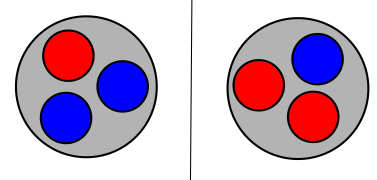
\includegraphics[width =5cm]{../images/mirror}
	\end{figure}
	\vspace{-25pt}
	\begin{figure}
		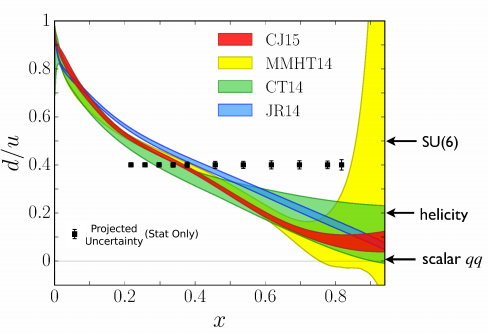
\includegraphics[width=5cm]{../images/d_u}
		\caption{d/u quark distribution ratios}
	\end{figure}
	
	\column{.55\textwidth} % Right column and width
	\begin{itemize}
		\item Lightest and simplest mirror system
		\begin{itemize}
			\item  Number of protons in $^3H =$ neutrons in $^3He$
		\end{itemize}
		\item Differences in the nuclear effects are small
		\item Improve the current measurement and understanding of $F^n_2/F^p_2$ ratio
		\item Restrict the assumptions and parameters made in the model calculations of the down to up quark distribution ratio
		\item 6 students from 4 universities
	\end{itemize}
	
	
\end{columns}
\end{frame}
%------------------------------------------------------------------
\section{Hall A at JLab}
\begin{frame}
\begin{block}{Jefferson Lab Hall A}
	\begin{figure}
		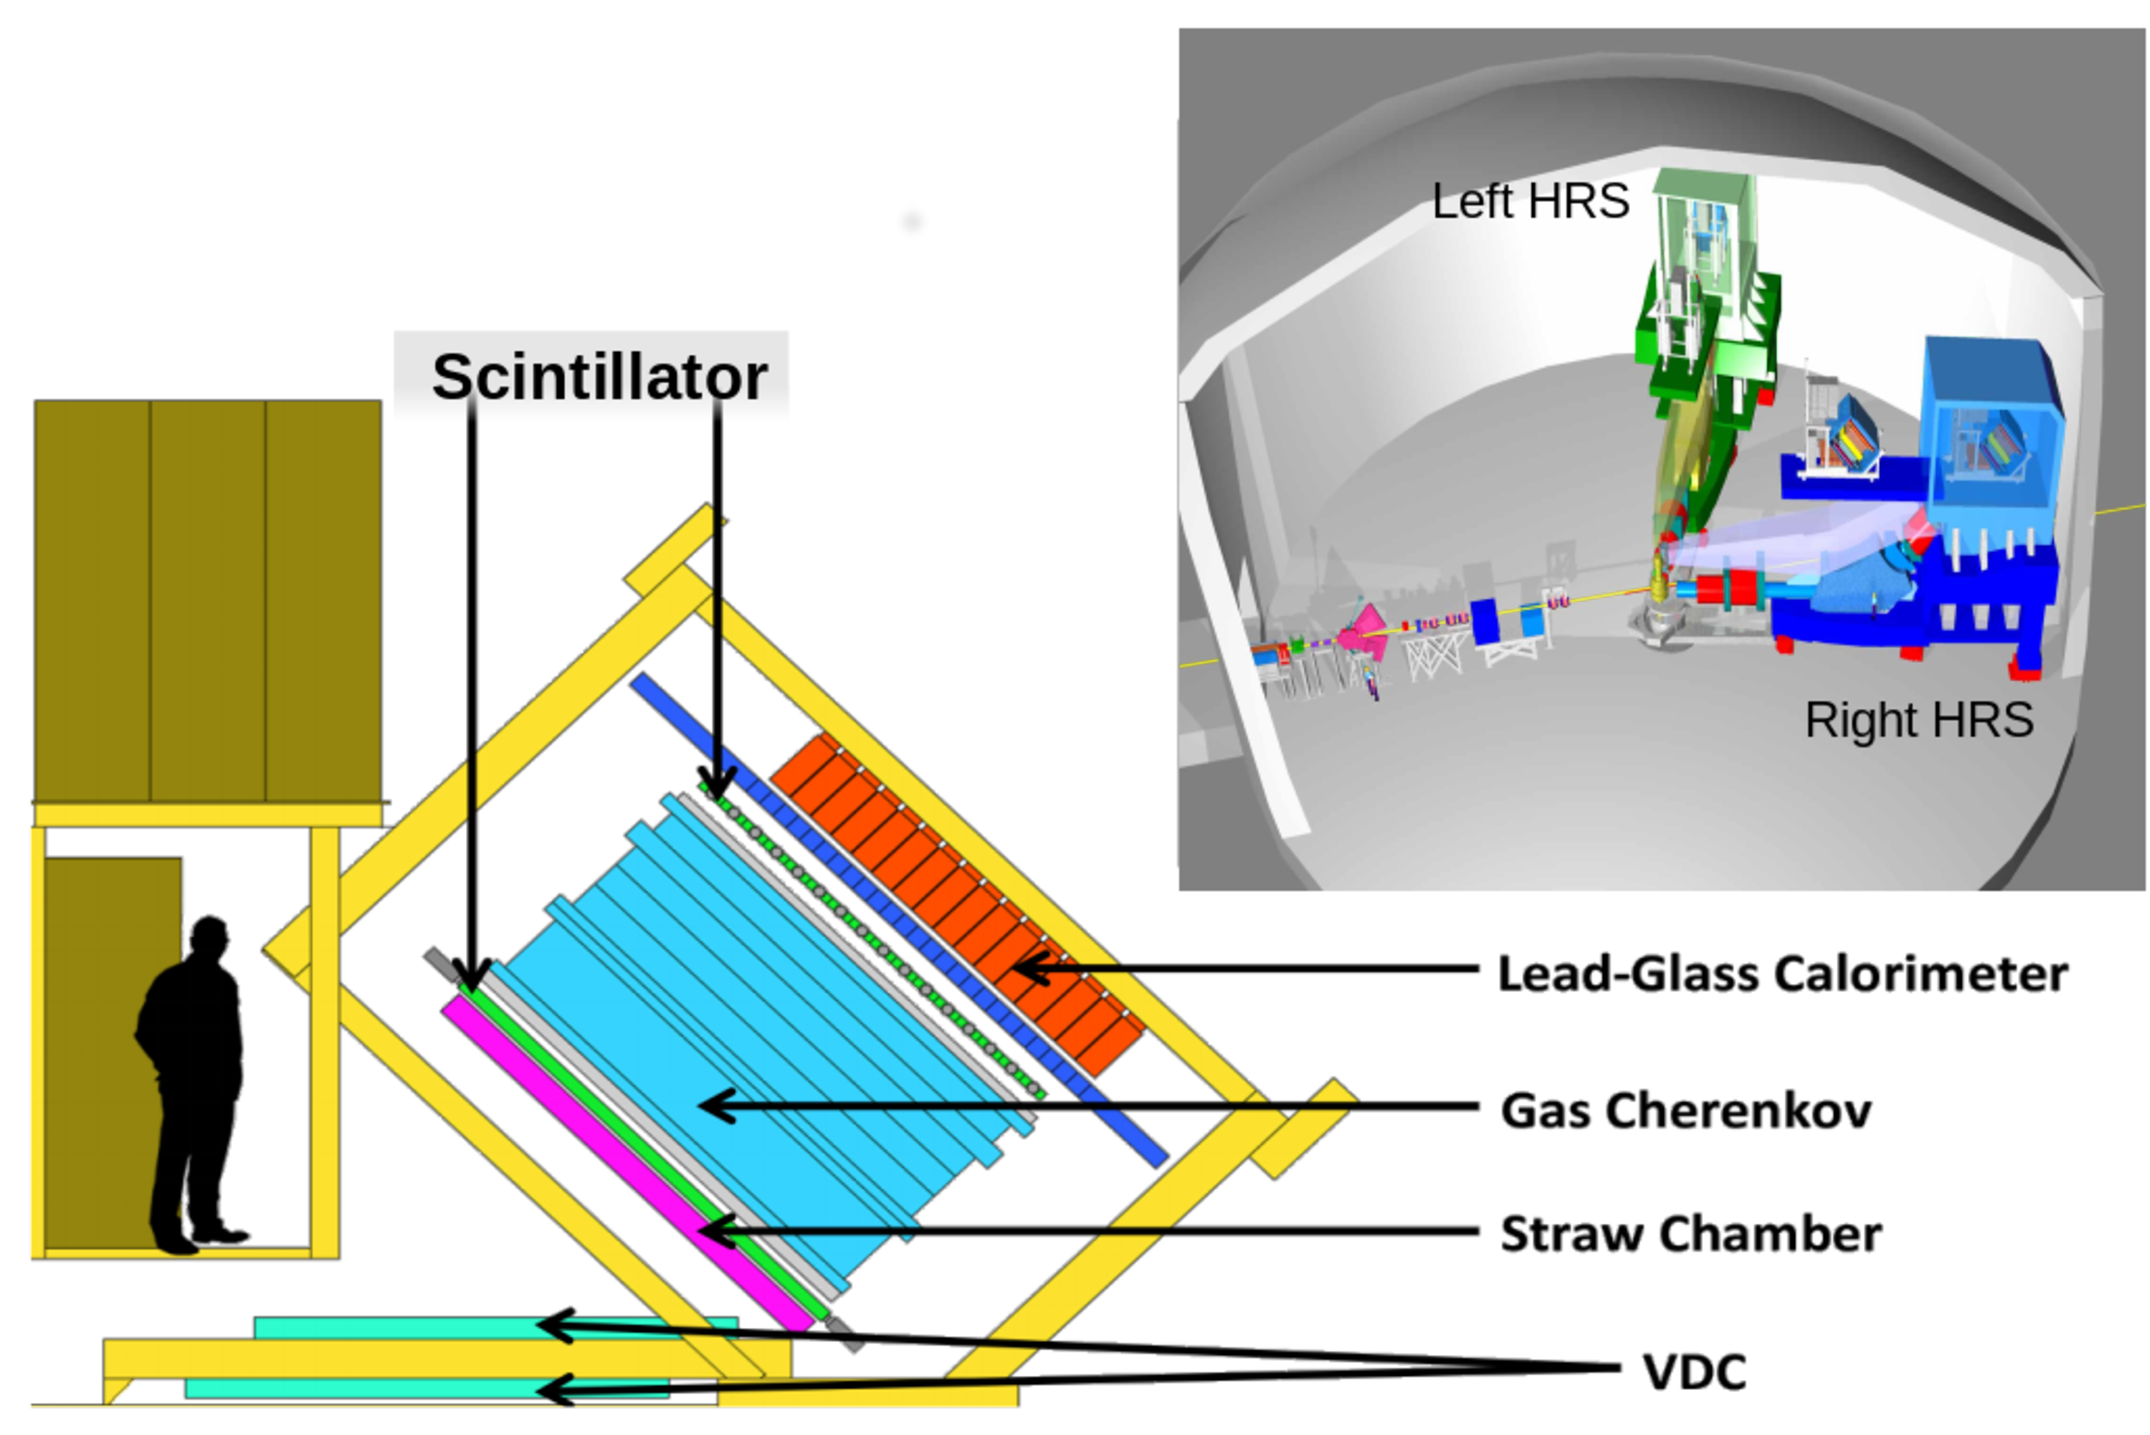
\includegraphics[width=12.0cm]{../images/HallaHRS.pdf}
	\end{figure}
	
\end{block}

\end{frame}
%------------------------------------------------------------------

\begin{frame}{Cross Section}
\begin{block}{}
	
	\centering
	$\frac{d\sigma}{d\Omega dE^\prime} =  \frac{Yield}{Luminosity} = \frac{Ne - BG }{Luminosity *  \epsilon} $
	
	\centering
	$N_e = \textit{L} * \left( \frac{d\sigma}{d\Omega dE^\prime} \right) * \left( \Delta E^\prime \Delta \Omega\right) \epsilon * A \left(E^\prime \theta \right)  + Back  Ground$
	
	\begin{itemize}
		\item $\textit{L}$ Luminosity $\equiv$ \# of electrons per scattering centers
		\item $\left( \Delta E^\prime \Delta \Omega\right) = $ size of bin
		\item $\epsilon = $ efficiencies
		\item  $A \left(E^\prime \theta \right) =$ Acceptance 
		
	\end{itemize}
	
	$ Yield_{data} = \frac{\left(N_e - BackGround\right)}{Efficency } =  \textit{L} *\sigma^{data} * \left( \Delta E^\prime \Delta \Omega\right)*  A \left(E^\prime \theta \right)$
	
	$ Yield_{MC} = \textit{L} *\sigma^{mod} * \left( \Delta E^\prime \Delta \Omega\right)*  A \left(E^\prime \theta \right)$
\end{block}



\begin{center}
	
	\begin{block}{}
		Cross section by Monte carlo ratio  method:
		\centering $ \frac{d\sigma}{d\Omega dE^\prime} = \sigma^{mod} * \left[\frac{Yield_{data} \left( 
			E^\prime,\theta\right)} {Yield_{MC}\left(E^\prime,\theta\right)}\right] $
		
	\end{block}	
\end{center}



\end{frame}
%------------------------------------------------------------------
\begin{frame}
\begin{columns}
\column{0.4\textwidth}
\begin{block}{Monte Carlo to Data}
	\begin{itemize}
		\item For Deuterium on kin15, we have 66 runs
		\item Use enough runs to average 10k events per bin
		\item monitoring the kinematic overlapping region
	\end{itemize}
\end{block}
\column{0.55\textwidth}
\vspace{-20pt}
\begin{figure}
	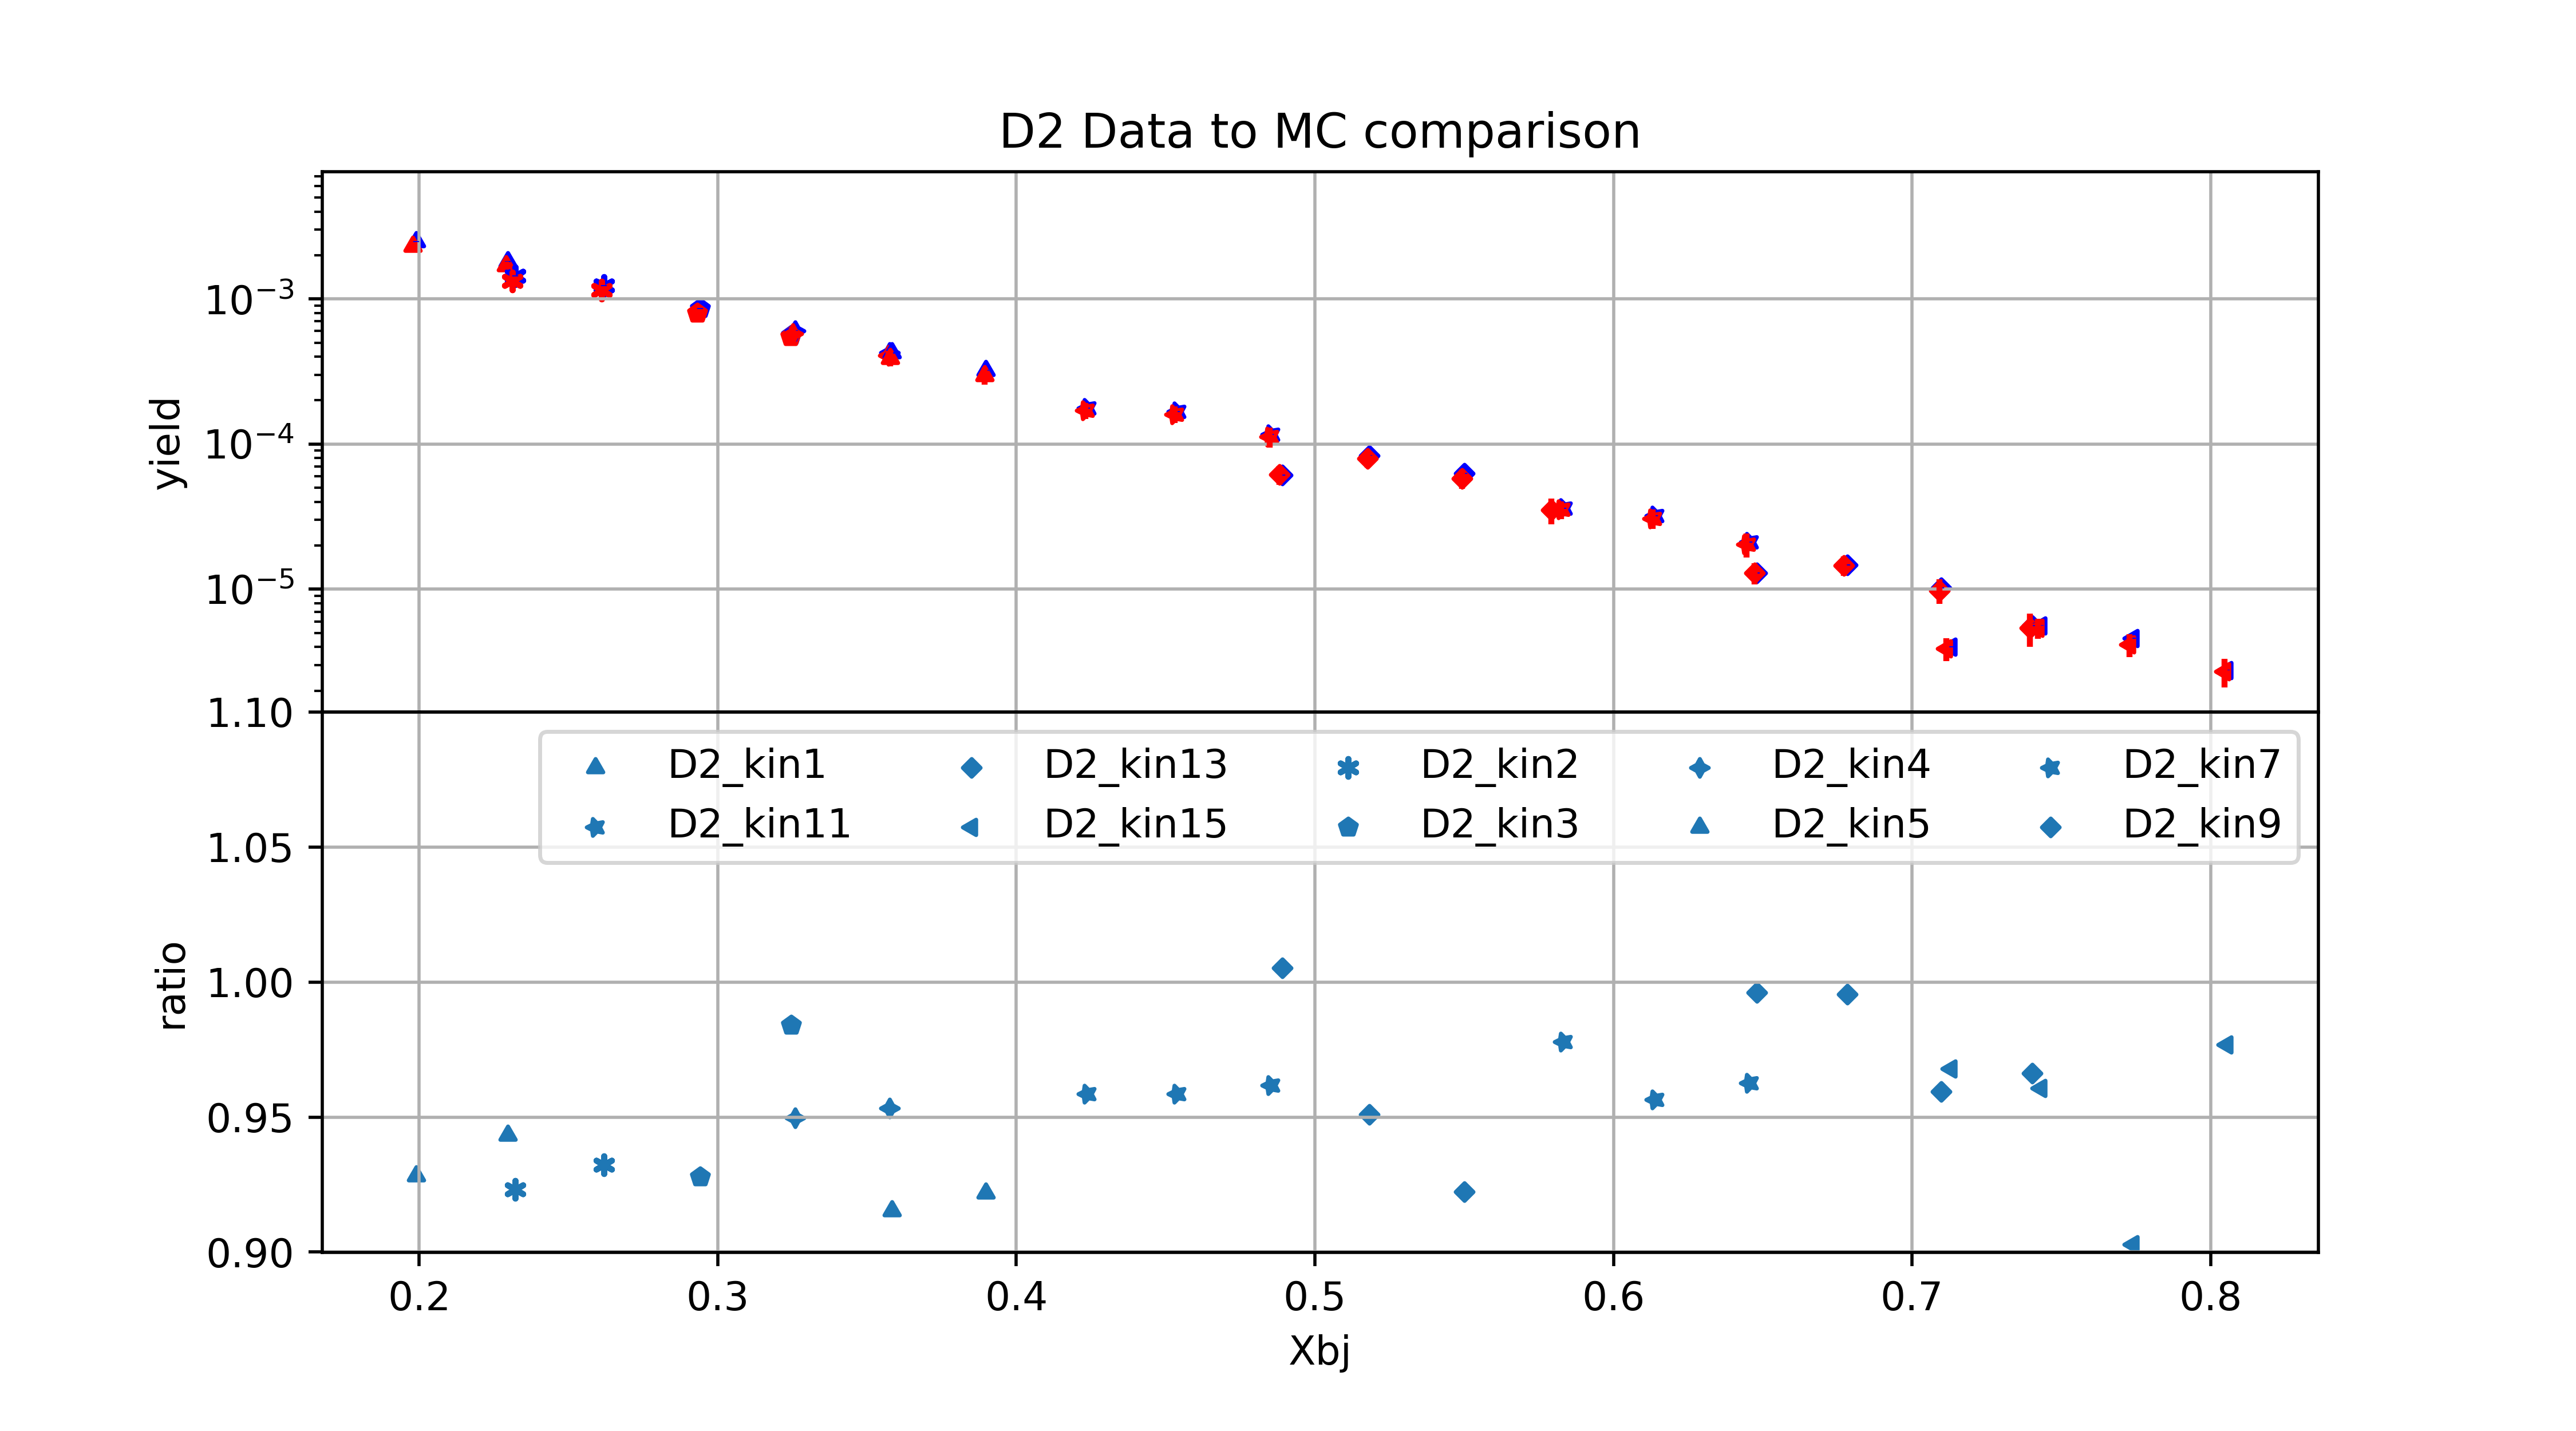
\includegraphics[width=7.5cm]{../images/D2_all}
\end{figure}
\vspace{-40pt}
\begin{figure}
	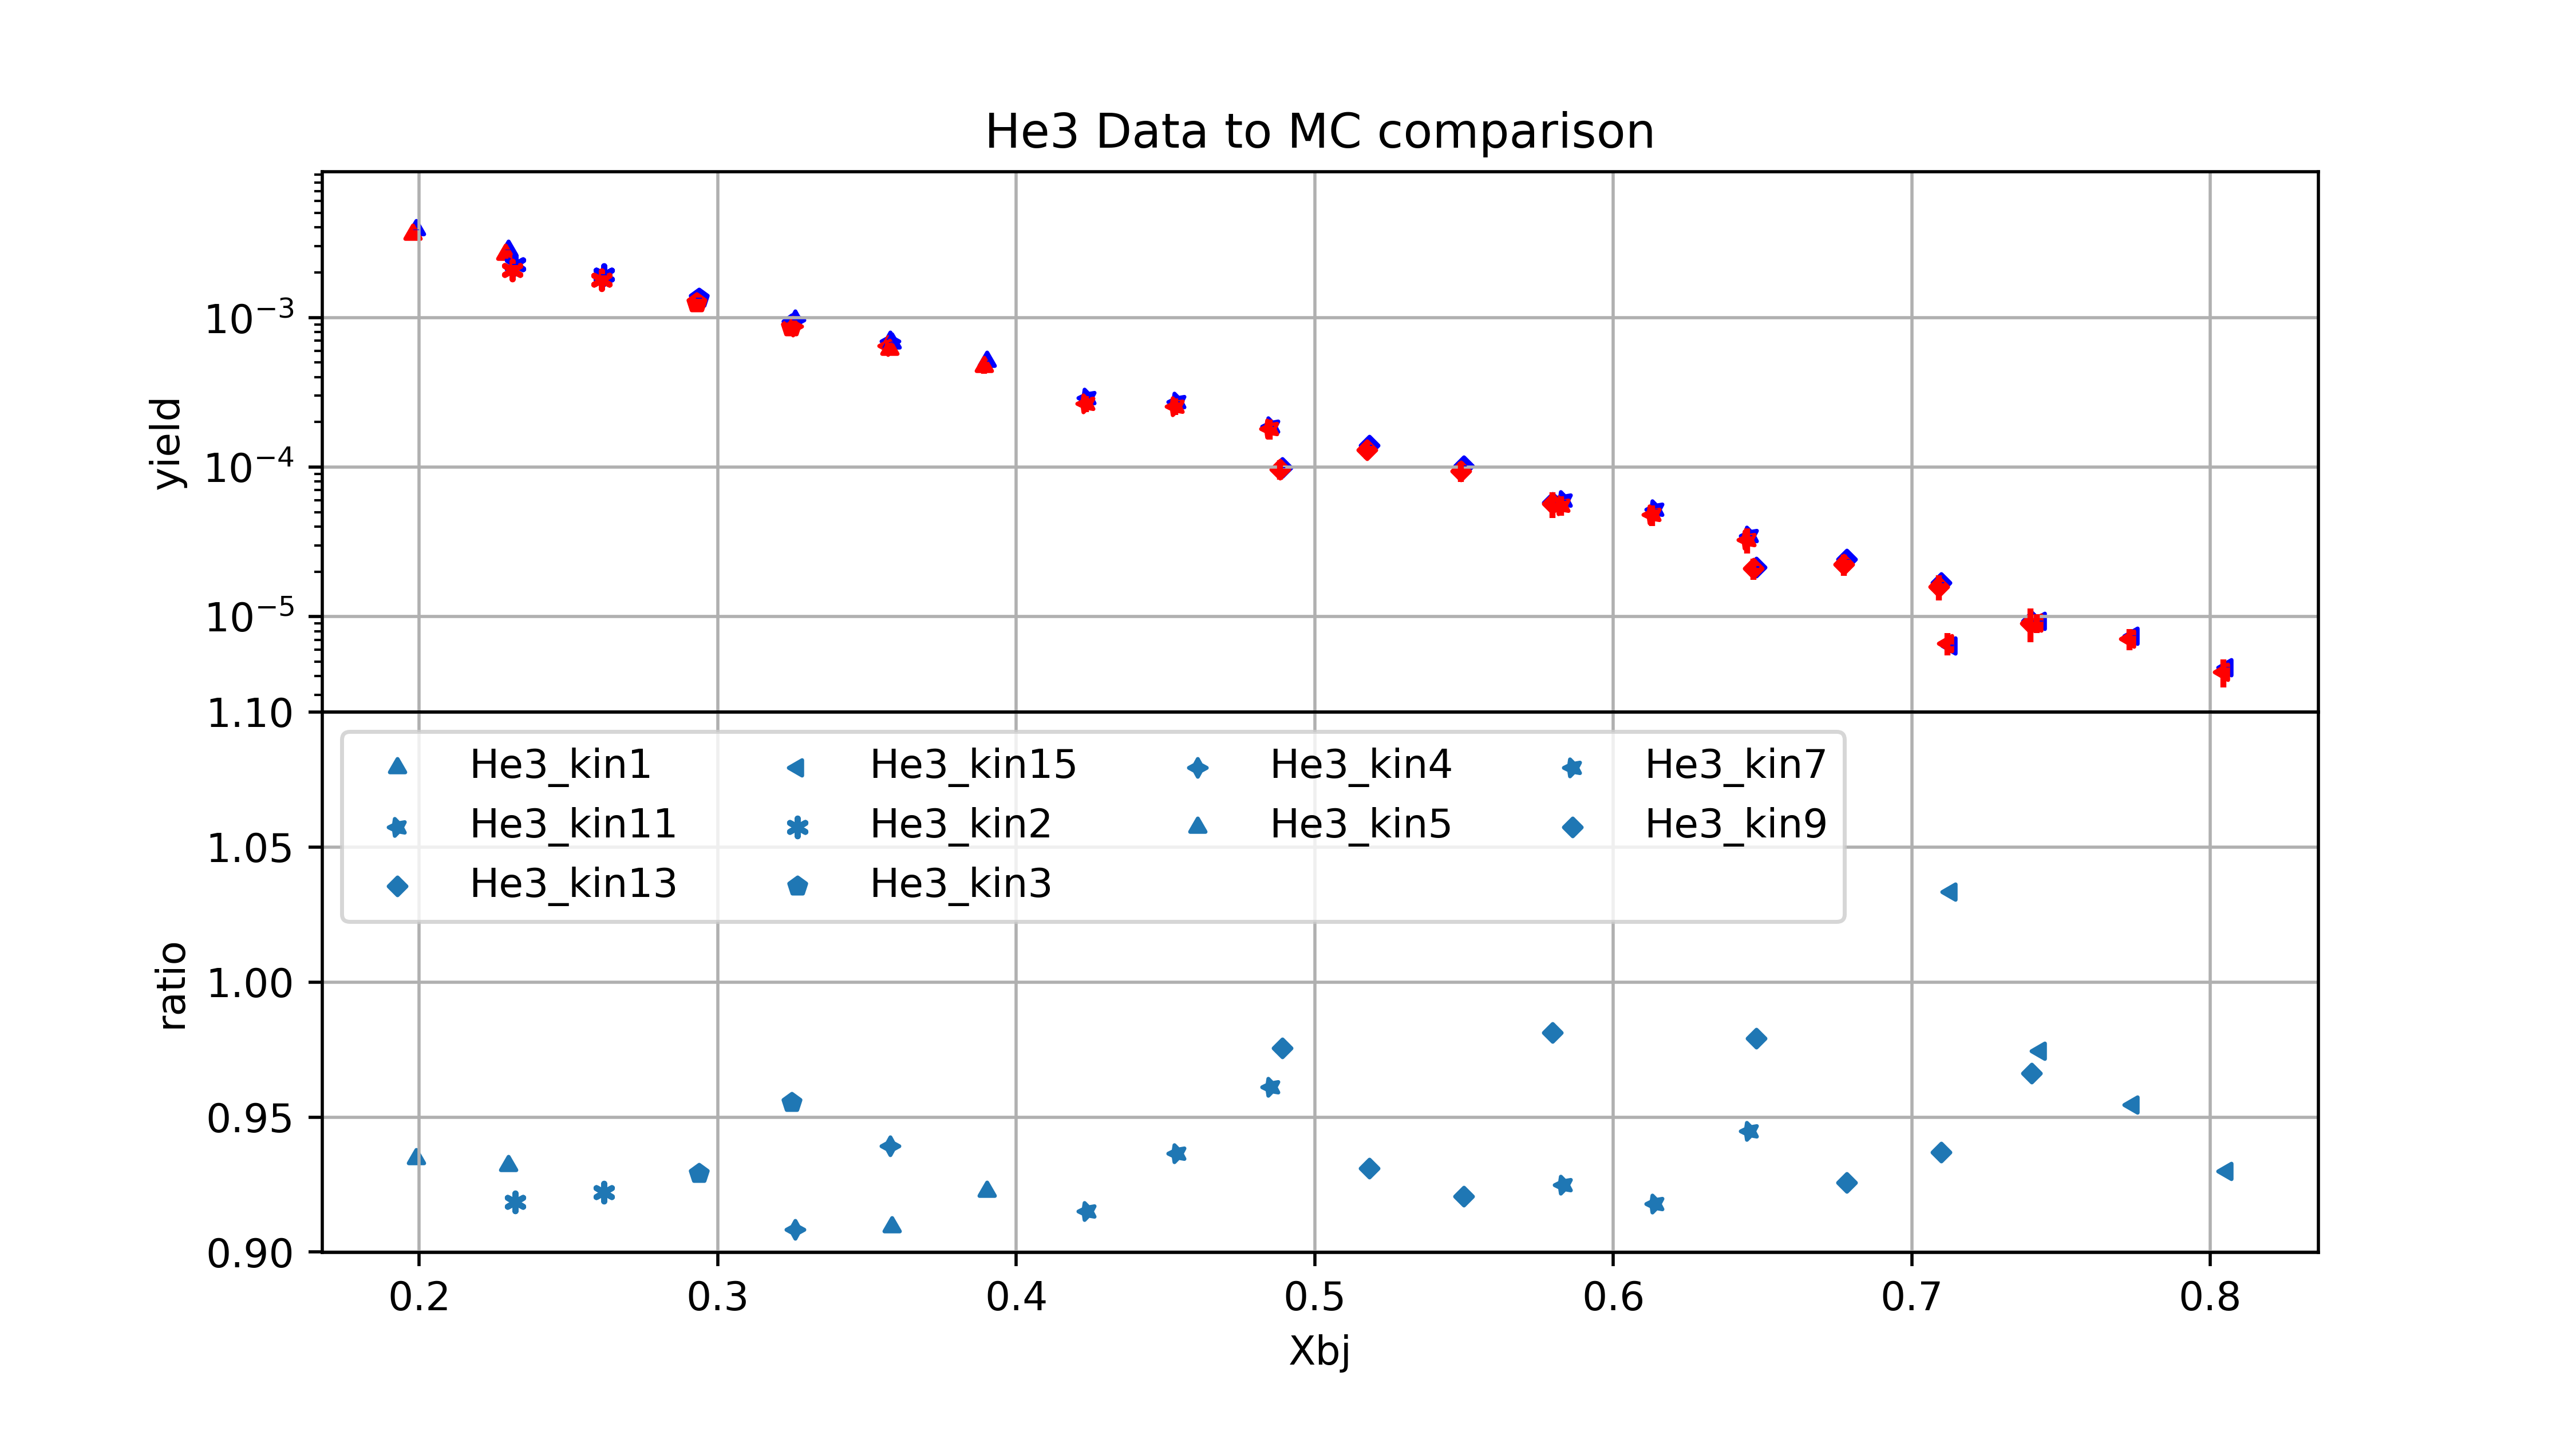
\includegraphics[width=7.5cm]{../images/He3_all}
\end{figure}
\end{columns}

\end{frame}

%------------------------------------------------------------------
\begin{frame}
\begin{block}{DIS (e,$e^\prime$) Cross section}
\begin{figure}
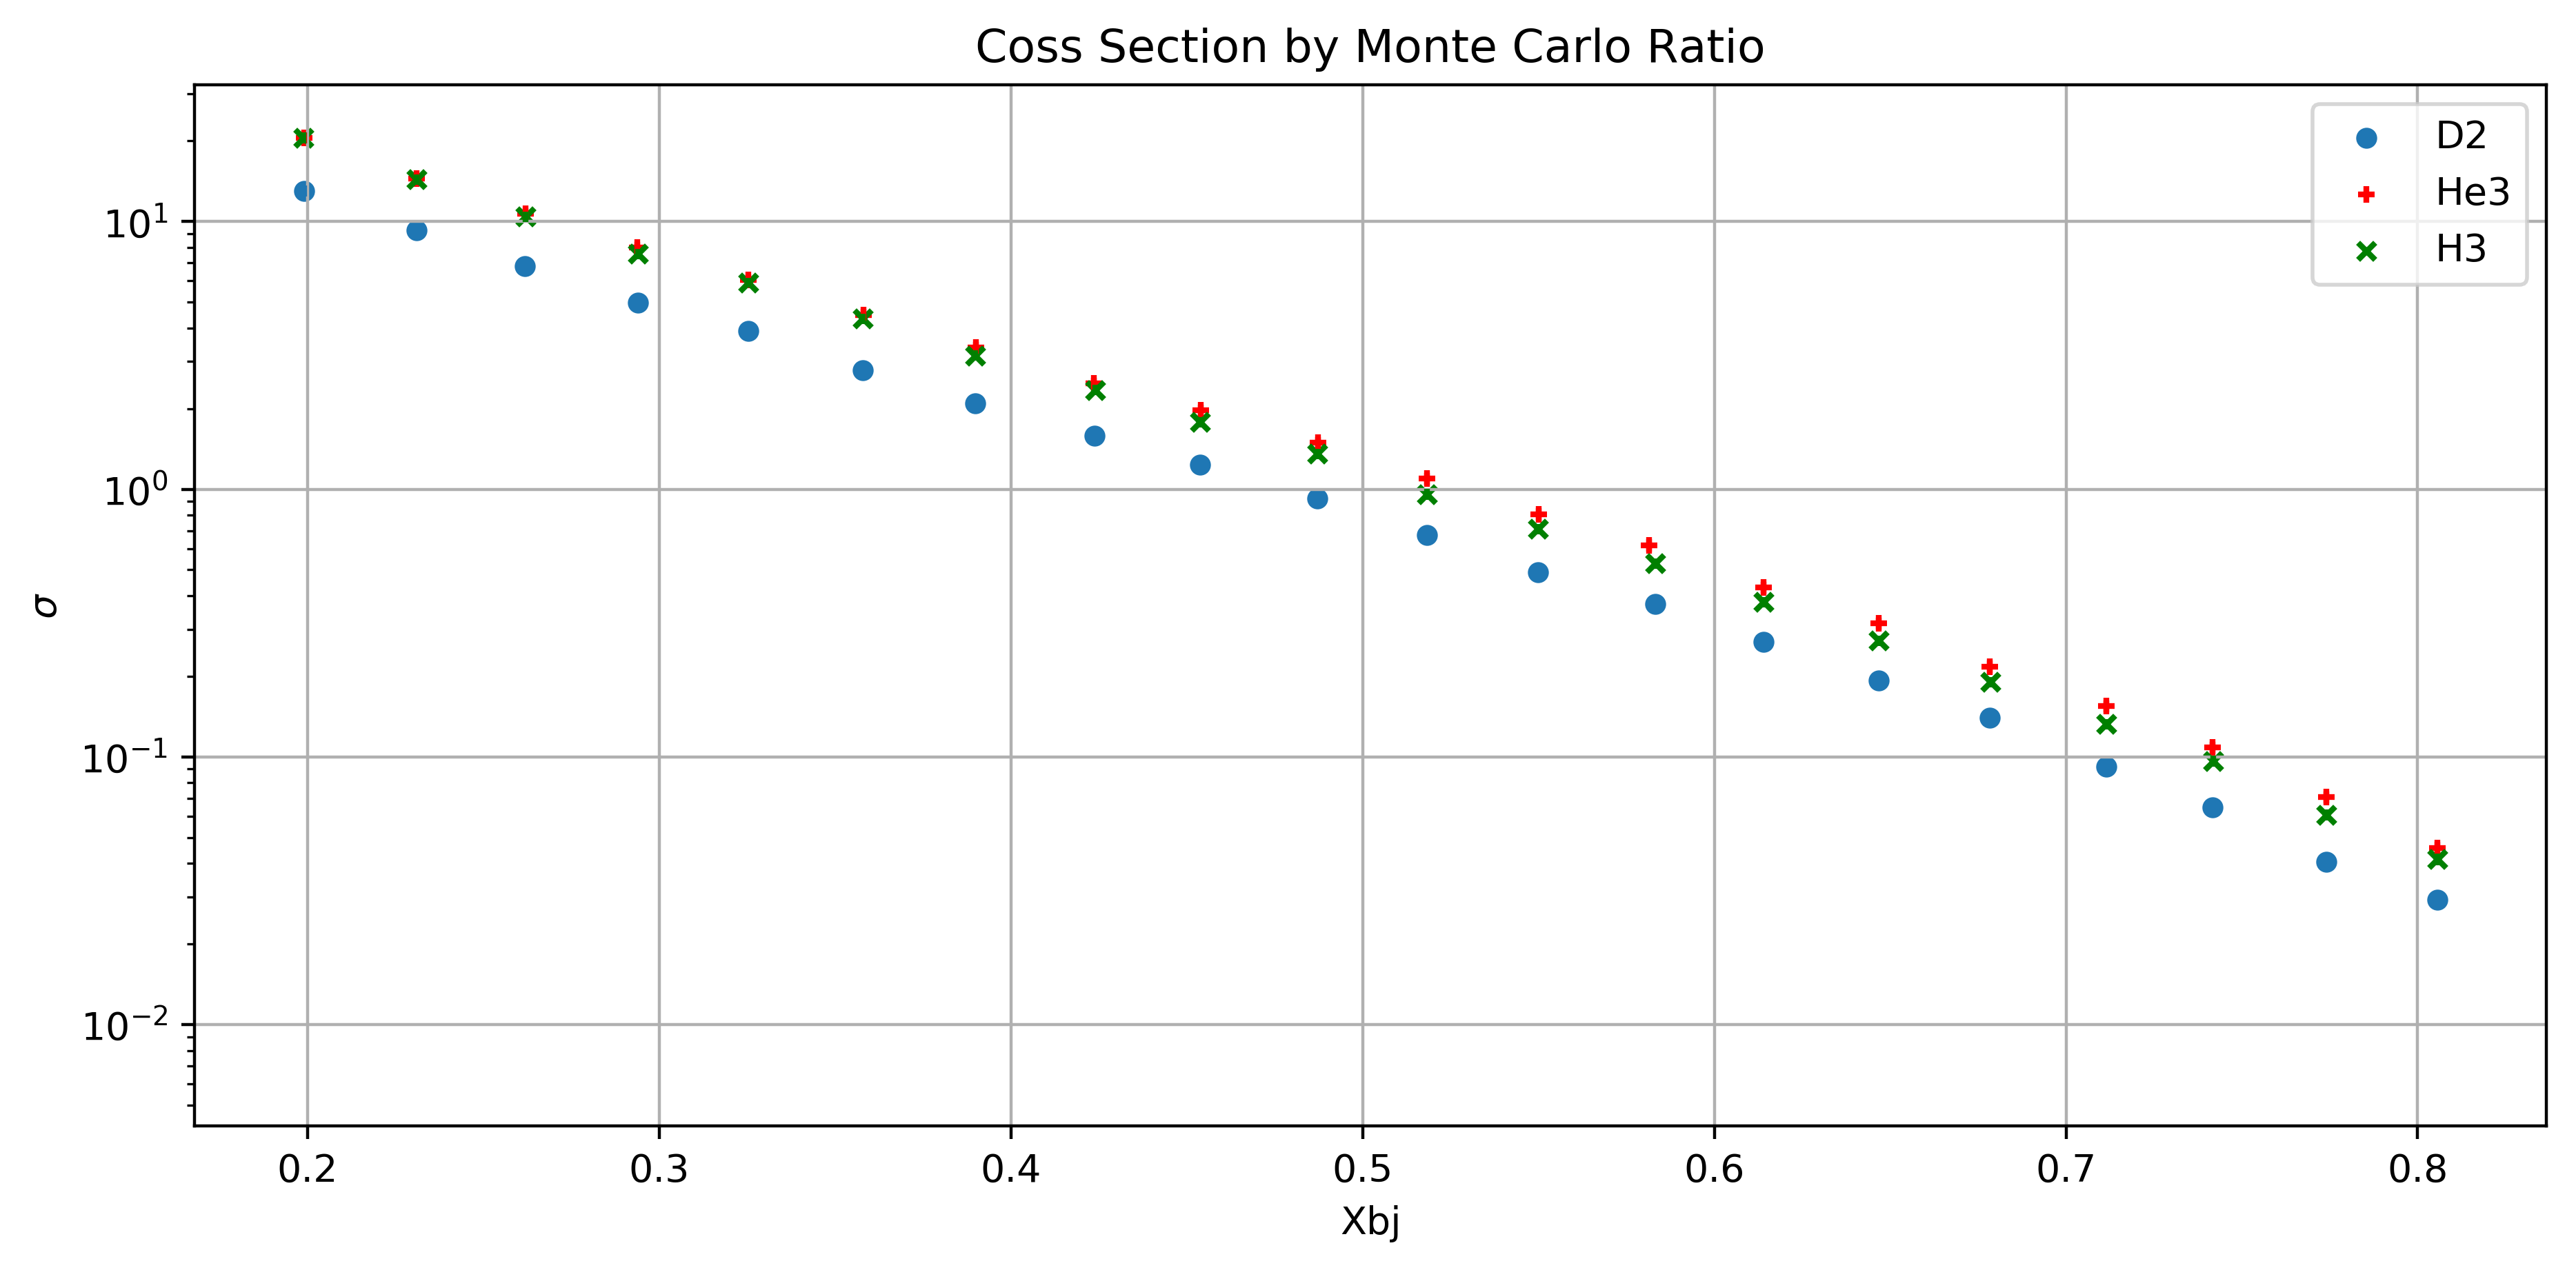
\includegraphics[width=12.0cm]{../images/all_final}
\end{figure}

\end{block}

\end{frame}

%------------------------------------------------------------------
\begin{frame}
\begin{block}{EMC effect}
\begin{figure}
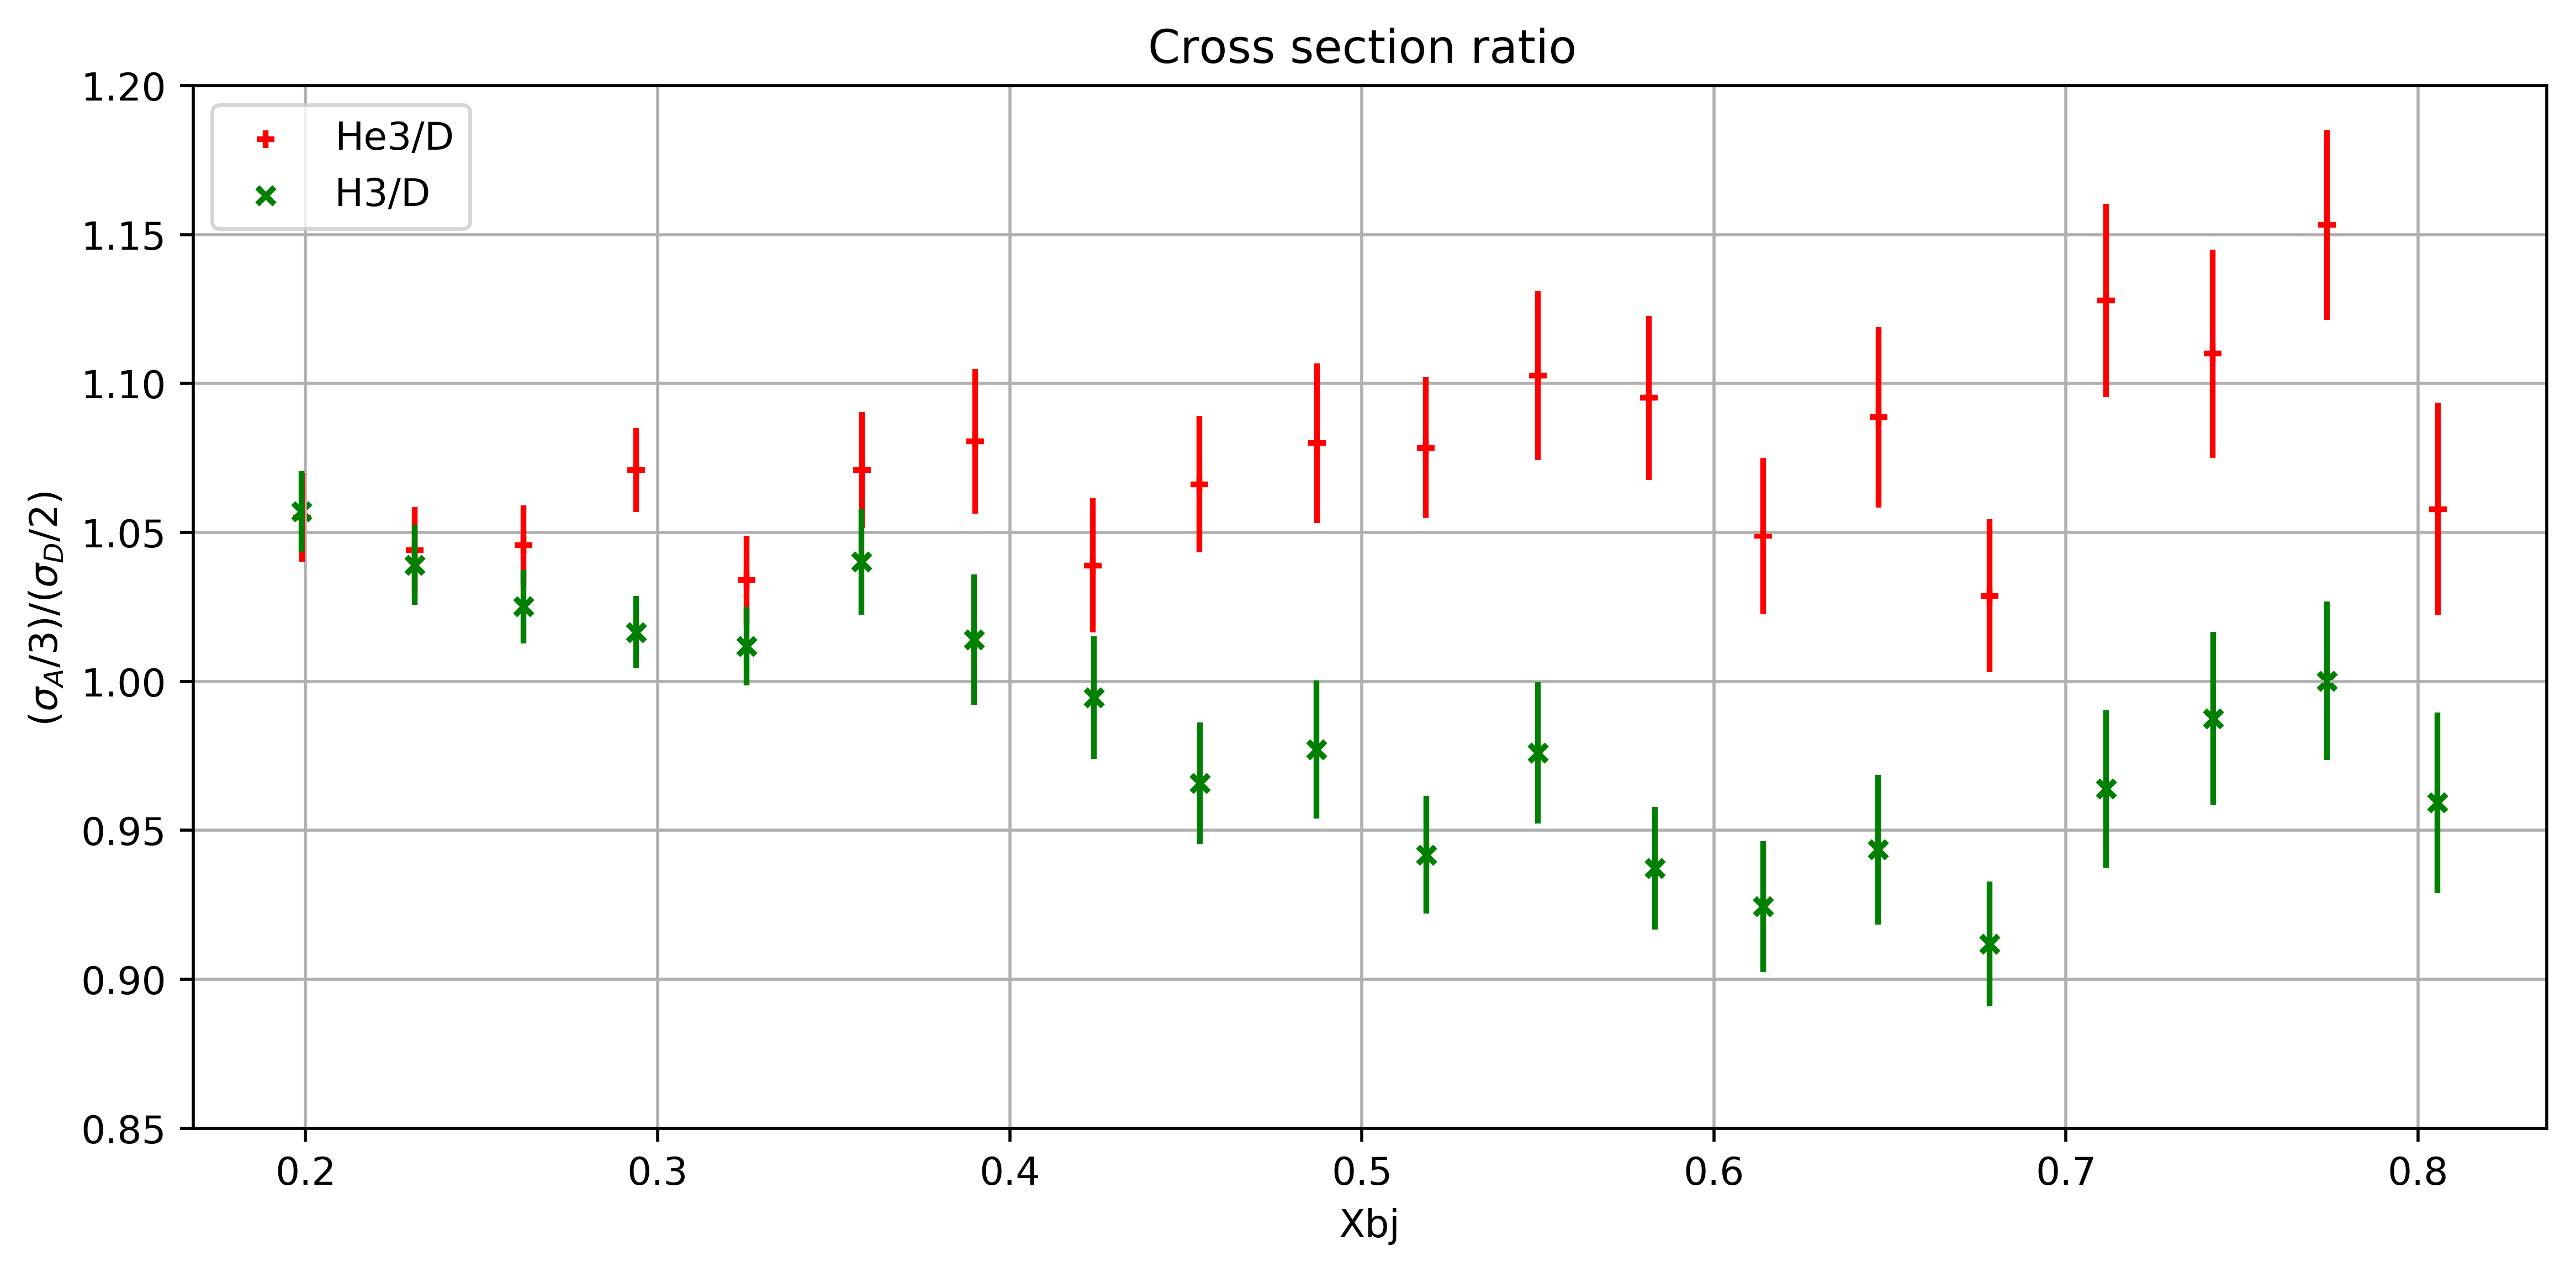
\includegraphics[width=12.0cm]{../images/EMC_final}
\end{figure}
\vspace{-20pt}
\begin{itemize}
\item Includes statistical error 
\item Need to add error from systematic studies

\end{itemize}

\end{block}

\end{frame}

%------------------------------------------------------------------

\end{document} 
